% ponytail: YAGNI! No macros with `#` inside a beamer frame to avoid fragile errors.

\begin{frame}[t]{Metodolgía: Resumen visual}
    \centering
    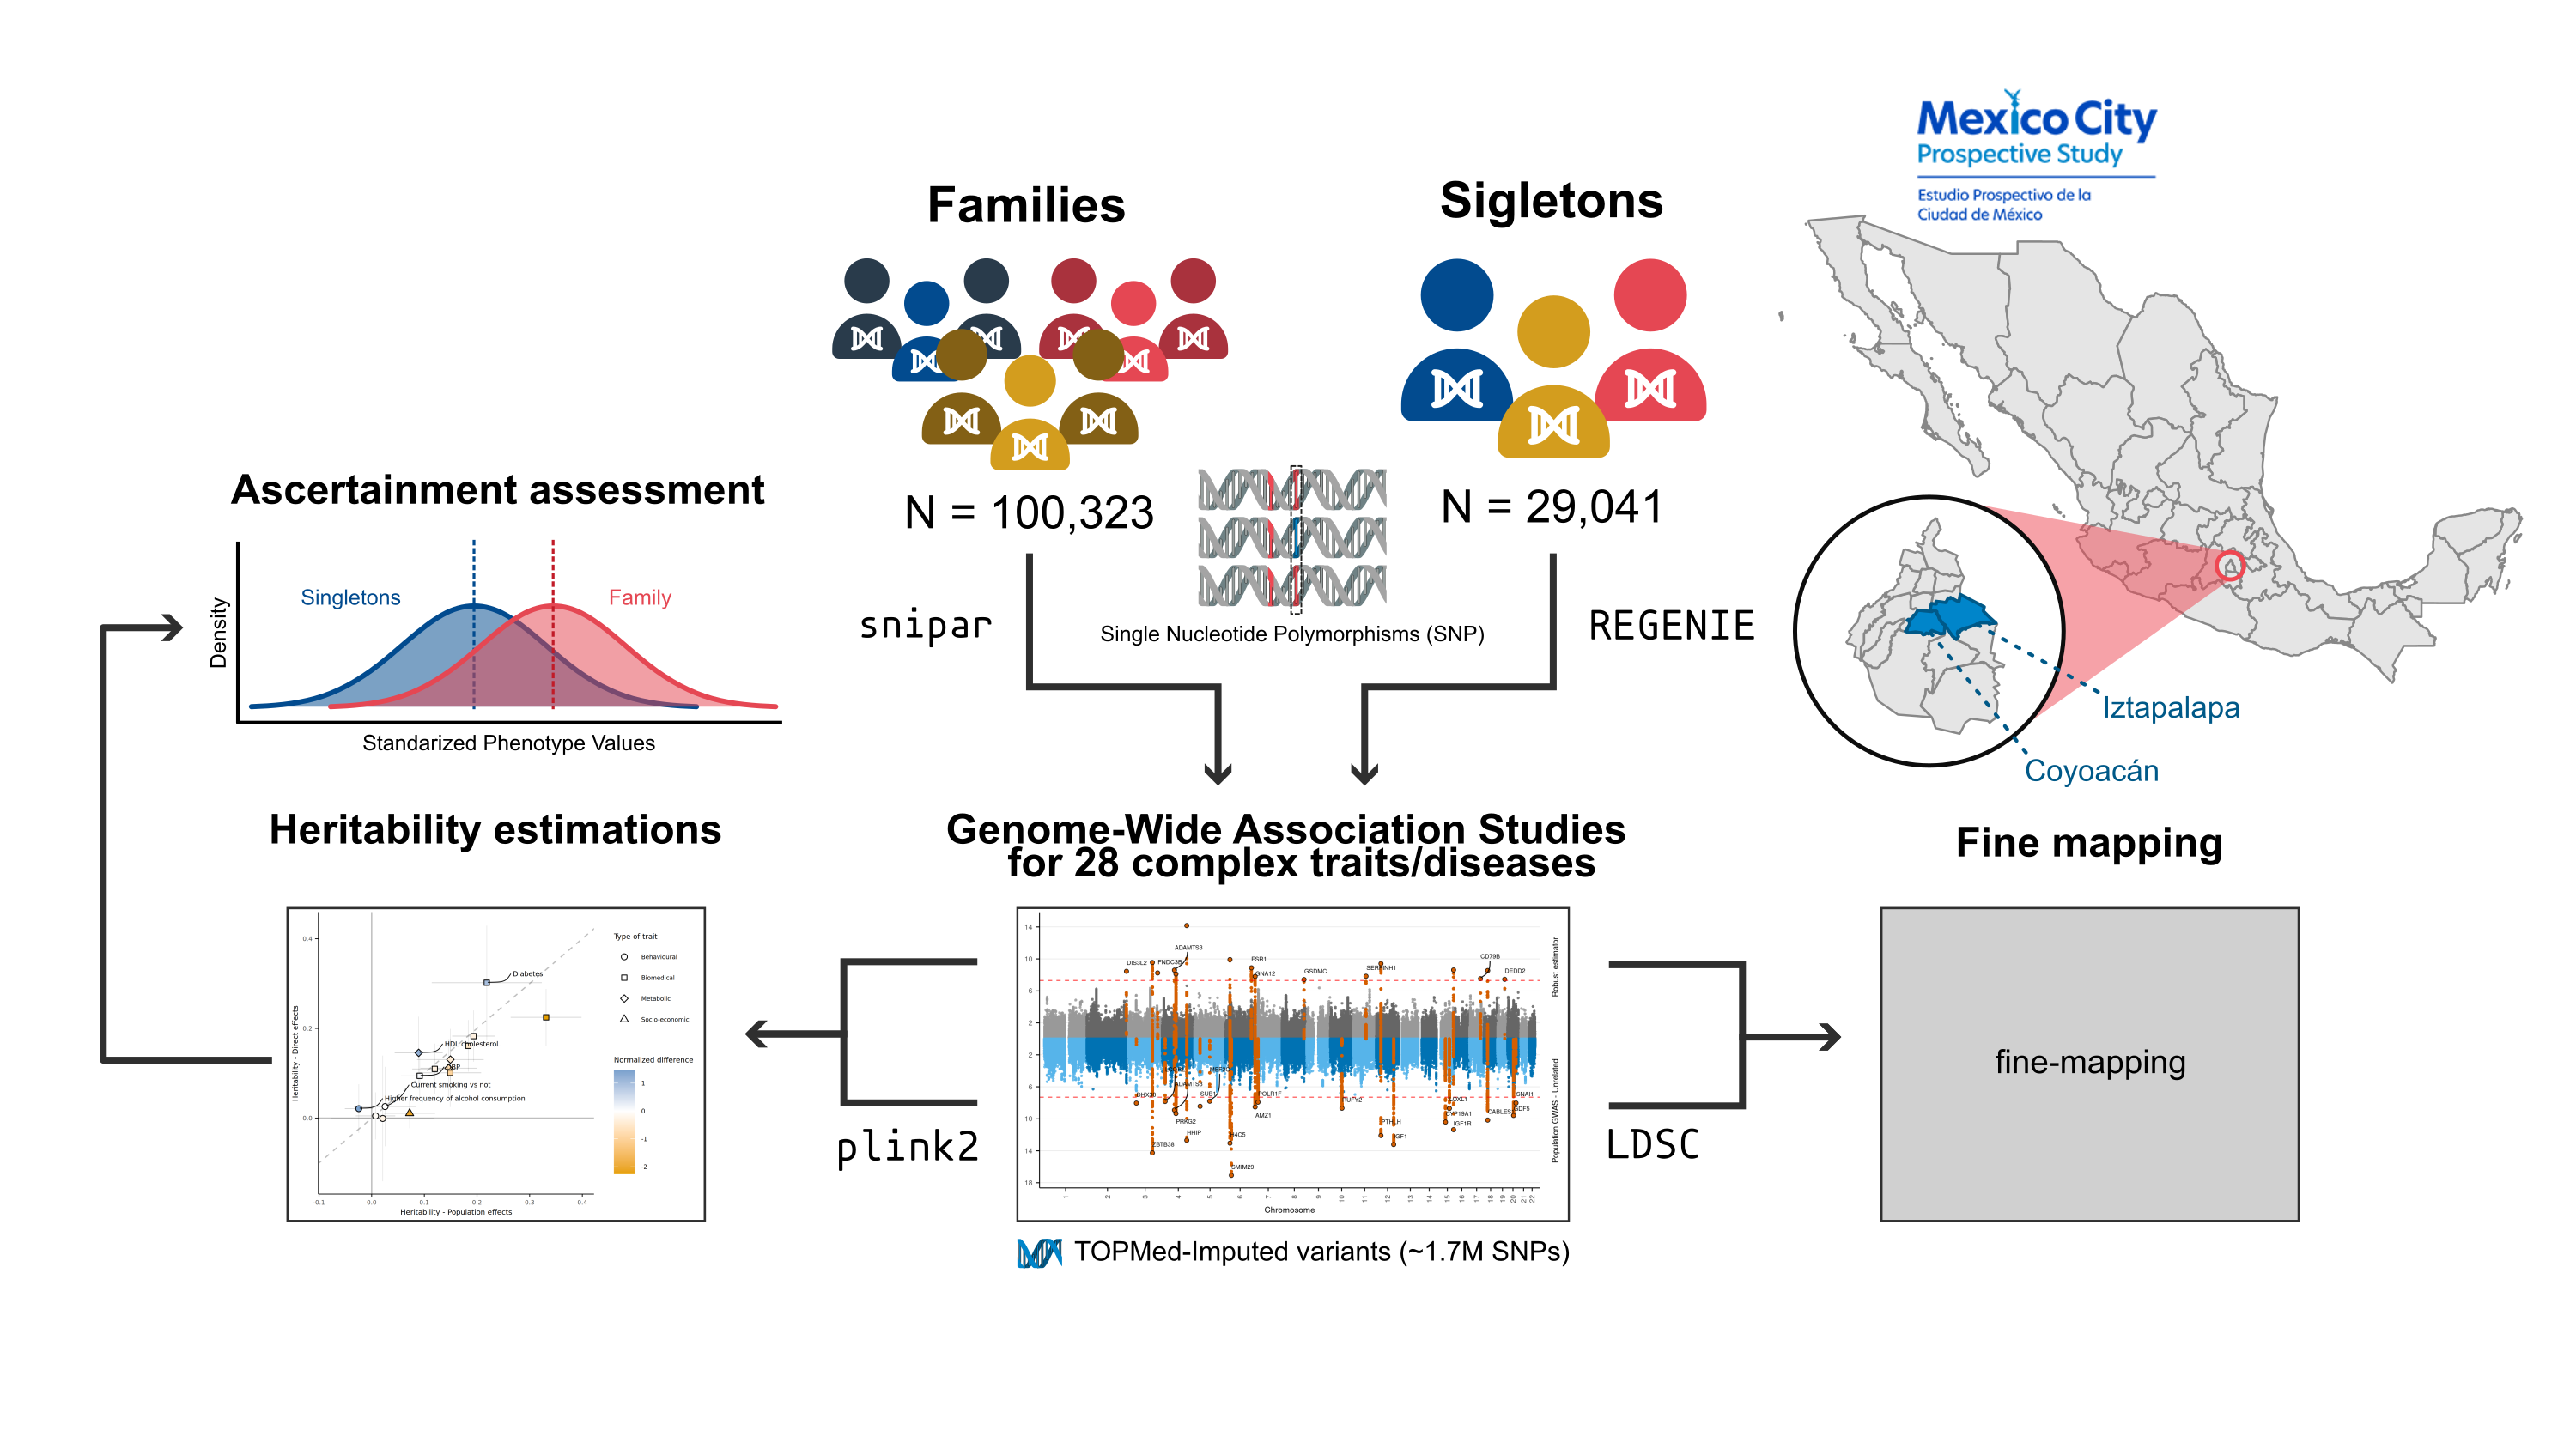
\includegraphics[height=\textheight]{img/diagrams/visual-abstract.png}
\end{frame}

% ---- Option C: Cascading Incremental ----
% ponytail: plain TikZ, no # args, hardcoded positions
\begin{frame}[b]{Diseño experimental: Escalamiento incremental}
\resizebox{!}{0.85\textheight}{
\centering
\begin{tikzpicture}

% ---- Column geometry (widening per semester) ----
% Labels
\def\lw{3.0}
% S1: x=3.15, w=1.5
% S2: x=4.85, w=2.2
% S3: x=7.25, w=3.0
% S4: x=10.45, w=3.4

% ---- Row y positions ----
% headers: 0.4
% scope: -0.15
% separator: -0.55
% IBD: -1.0
% Imp: -1.65
% FGWAS: -2.3
% LDSC: -2.95
% PRS: -3.6

\def\barH{0.45}

% ==== SEMESTER HEADERS ====
\node[fill=ccgblue, text=white, font=\footnotesize\bfseries, rounded corners=2pt, minimum width=2.45cm, minimum height=0.45cm] at (4.375, 0.4) {S1};
\node[fill=unamgold, text=white, font=\footnotesize\bfseries, rounded corners=2pt, minimum width=2.45cm, minimum height=0.45cm] at (7.125, 0.4) {S2};
\node[fill=green, text=white, font=\footnotesize\bfseries, rounded corners=2pt, minimum width=2.45cm, minimum height=0.45cm] at (9.875, 0.4) {S3};
\node[fill=red, text=white, font=\footnotesize\bfseries, rounded corners=2pt, minimum width=2.45cm, minimum height=0.45cm] at (12.625, 0.4) {S4};

% ==== SCOPE: 3-row icon grid ====
% Row 1: Database (\faDatabase)
\node[font=\footnotesize, text=black!50, anchor=east] at (2.9, -0.1) {\faDatabase};
\node[font=\scriptsize, text=ccgblue] at (4.375, -0.1)  {GSAv2 CHIP};
\node[font=\scriptsize, text=unamgold] at (7.125, -0.1) {TOPMed Imputed};
\node[font=\scriptsize, text=green] at (9.875, -0.1)    {TOPMed Imputed};
\node[font=\scriptsize, text=red] at (12.625, -0.1)     {TOPMed Imputed};

% Row 2: Chromosomes (\faDna)
\node[font=\footnotesize, text=black!50, anchor=east] at (2.9, -0.4) {\faDna};
\node[font=\scriptsize, text=ccgblue] at (4.375, -0.4)  {Chr. 22};
\node[font=\scriptsize, text=unamgold] at (7.125, -0.4) {Chr. 1--22};
\node[font=\scriptsize, text=green] at (9.875, -0.4)    {Chr. 1--22};
\node[font=\scriptsize, text=red] at (12.625, -0.4)     {Chr. 1--22};

% Row 3: Traits (\faHeartbeat)
\node[font=\scriptsize, text=black!50, anchor=east] at (2.9, -0.7) {\faHeartbeat};
\node[font=\scriptsize, text=ccgblue] at (4.375, -0.7) {3 rasgos};
\node[font=\scriptsize, text=unamgold] at (7.125, -0.7) {13 rasgos};
\node[font=\scriptsize, text=green] at (9.875, -0.7) {17 rasgos};
\node[font=\scriptsize, text=red] at (12.625, -0.7) {28 rasgos};

% ==== SEPARATOR LINE ====
\draw[gray!40, thin] (0, -1.0) -- (13.85, -1.0);

% ==== ROW LABELS ====
\node[font=\scriptsize, anchor=east] at (2.9, -1.4) {IBD entre hermanos};
\node[font=\scriptsize, anchor=east] at (2.9, -2.0) {Imputación Mendeliana};
\node[font=\scriptsize, anchor=east] at (2.9, -2.6) {GWAS (REGENIE)};
\node[font=\scriptsize, anchor=east] at (2.9, -3.2) {FGWAS (\textit{Sibpair/Trios})};
\node[font=\scriptsize, anchor=east] at (2.9, -3.8) {FGWAS (\textit{Imputed})};
\node[font=\scriptsize, anchor=east] at (2.9, -4.4) {FGWAS (\textit{Robust estimator})};
\node[font=\scriptsize, anchor=east] at (2.9, -5.0) {Correlaciones genéticas \& Heredabilidad};
\node[font=\scriptsize, anchor=east] at (2.9, -5.6) {Fine-mapping};

% ==== BARS ====
% --- IBD ---
\draw[gray!20, dashed, rounded corners=2pt] (3.15, {-1.4-\barH/2}) rectangle (5.6, {-1.4+\barH/2});
\fill[unamgold!70, rounded corners=2pt] (5.9, {-1.4-\barH/2}) rectangle (8.35, {-1.4+\barH/2});
\node[font=\tiny, text=black!40] at (9.875, -1.4) {\faCheck};
\node[font=\tiny, text=black!40] at (12.625, -1.4) {\faCheck};

% --- Imputación ---
\draw[gray!20, dashed, rounded corners=2pt] (3.15, {-2.0-\barH/2}) rectangle (5.6, {-2.0+\barH/2});
\fill[unamgold!70, rounded corners=2pt] (5.9, {-2.0-\barH/2}) rectangle (8.35, {-2.0+\barH/2});
\node[font=\tiny, text=black!40] at (9.875, -2.0) {\faCheck};
\node[font=\tiny, text=black!40] at (12.625, -2.0) {\faCheck};

% --- GWAS ---
\draw[gray!20, dashed, rounded corners=2pt] (3.15, {-2.6-\barH/2}) rectangle (5.6, {-2.6+\barH/2});
\draw[gray!20, dashed, rounded corners=2pt] (5.9, {-2.6-\barH/2}) rectangle (8.35, {-2.6+\barH/2});
\fill[green!70, rounded corners=2pt] (8.65, {-2.6-\barH/2}) rectangle (11.1, {-2.6+\barH/2});
\fill[red!70, rounded corners=2pt] (11.4, {-2.6-\barH/2}) rectangle (13.85, {-2.6+\barH/2});

% --- FGWAS (est. 1): S1 only ---
\fill[ccgblue!50, rounded corners=2pt] (3.15, {-3.2-\barH/2}) rectangle (5.6, {-3.2+\barH/2});
\draw[gray!20, dashed, rounded corners=2pt] (5.9, {-3.2-\barH/2}) rectangle (8.35, {-3.2+\barH/2});
\draw[gray!20, dashed, rounded corners=2pt] (8.65, {-3.2-\barH/2}) rectangle (11.1, {-3.2+\barH/2});
\draw[gray!20, dashed, rounded corners=2pt] (11.4, {-3.2-\barH/2}) rectangle (13.85, {-3.2+\barH/2});

% --- FGWAS (est. 2): S1, S2 ---
\fill[ccgblue!50, rounded corners=2pt] (3.15, {-3.8-\barH/2}) rectangle (5.6, {-3.8+\barH/2});
\fill[unamgold!70, rounded corners=2pt] (5.9, {-3.8-\barH/2}) rectangle (8.35, {-3.8+\barH/2});
\draw[gray!20, dashed, rounded corners=2pt] (8.65, {-3.8-\barH/2}) rectangle (11.1, {-3.8+\barH/2});
\draw[gray!20, dashed, rounded corners=2pt] (11.4, {-3.8-\barH/2}) rectangle (13.85, {-3.8+\barH/2});

% --- FGWAS (est. 3): S3, S4 ---
\draw[gray!20, dashed, rounded corners=2pt] (3.15, {-4.4-\barH/2}) rectangle (5.6, {-4.4+\barH/2});
\draw[gray!20, dashed, rounded corners=2pt] (5.9, {-4.4-\barH/2}) rectangle (8.35, {-4.4+\barH/2});
\fill[green!70, rounded corners=2pt] (8.65, {-4.4-\barH/2}) rectangle (11.1, {-4.4+\barH/2});
\fill[red!70, rounded corners=2pt] (11.4, {-4.4-\barH/2}) rectangle (13.85, {-4.4+\barH/2});

% --- Correlaciones genéticas & Heredabilidad ---
\draw[gray!20, dashed, rounded corners=2pt] (3.15, {-5.0-\barH/2}) rectangle (5.6, {-5.0+\barH/2});
\fill[unamgold!70, rounded corners=2pt] (5.9, {-5.0-\barH/2}) rectangle (8.35, {-5.0+\barH/2});
\fill[green!70, rounded corners=2pt] (8.65, {-5.0-\barH/2}) rectangle (11.1, {-5.0+\barH/2});
\fill[red!70, rounded corners=2pt] (11.4, {-5.0-\barH/2}) rectangle (13.85, {-5.0+\barH/2});

% --- Fine-mapping: S4 only ---
\draw[gray!20, dashed, rounded corners=2pt] (3.15, {-5.6-\barH/2}) rectangle (5.6, {-5.6+\barH/2});
\draw[gray!20, dashed, rounded corners=2pt] (5.9, {-5.6-\barH/2}) rectangle (8.35, {-5.6+\barH/2});
\draw[gray!20, dashed, rounded corners=2pt] (8.65, {-5.6-\barH/2}) rectangle (11.1, {-5.6+\barH/2});
\fill[red!70, rounded corners=2pt] (11.4, {-5.6-\barH/2}) rectangle (13.85, {-5.6+\barH/2});

% ==== BOTTOM ARROW showing progression ====
\draw[-{Stealth[length=3mm]}, thick, gray!50] (3.15, -6.3) -- (13.85, -6.3);
\node[font=\footnotesize, text=gray!60, anchor=north] at (8.5, -6.35) {Alcance incremental};

\end{tikzpicture}
}
\end{frame}